\documentclass[12]{scrartcl}

\usepackage[normalem]{ulem}
\usepackage[utf8]{inputenc}

\usepackage{amsmath,amssymb,amstext}

% figures
\usepackage{caption}
\usepackage{subcaption}
\usepackage{float}

\usepackage{graphicx}
\usepackage{tikz}
\usepackage{cite}

\begin{document}


\begin{titlepage}
	\centering
	{\scshape\LARGE University of Zürich\par}
	\vspace{1cm}
	{\scshape\Large Distributed Database\par}
	\vspace{1.5cm}
	{\huge\bfseries Communication Cost Comparison in 3-Site Semi-Join using Composite Bloom Filters\par}
	\vspace{2cm}
	{\Large Andreas Schaufelbühl, Mirko Richter\par}
	\vfill
	
	% Bottom of the page
	{\large \today\par}
\end{titlepage}

\tableofcontents
\listoffigures
\listoftables
	
\section{Introduction}
The basis for this project is a paper from Michael {\em et al}\cite{michael} that gives extensions of bloom filters from basic two-sites database joins to settings with multiple sites. Generally, in a distributed database setting bloom filters can be used to reduce the communication costs. Bloom filters can represent a dataset in a compressed way by hashing the data into a bit array, which we call the bloom filter. The result of hashing a data point gives the index or indices in the bit array which corresponds to this data point. This leads to two important properties of bloom filters. First, bloom filters can not be used to send data from one site to another. It rather represents a set of data points such that at a different site one can verify whether a given data point is included in the bloom filter or not. Secondly, when used for verifying whether a given data point is in a bloom filter, the bloom filter can actually give a false positive. Meaning, it claims that this data point is included in the set while it actually is not. As a result, it is not always advisable to use bloom filters. Michael (2007) shows us that there are three variables which contribute to the probability that a bloom filter return a false positive. First, the amount of data to be represented matters as well as the size or length of the bloom filter and the number of hash functions used. The paper already suggests an optimal relation between those variables for a simple bloom filter join between two sites and it goes on an shows how the bloom filters can be combined when there are multiple sites such that one can reduce communication cost even further. This leads us to our project where we set up an experiment to verify some claims made in Michael {\em et al}\cite{michael}.

\section{Problem Description}
A join in a distributed database setting can lead to a lot of communication between the different sites. To reduce the communication cost, one can use bloom filters instead of sending the data points plainly. But since bloom filters do not contain data points but only a representation of them and can return false positives, it is not obvious that a join with bloom filters will perform better.\\\\
Michael (2007) provides an optimal relation
\begin{equation}
	k \approx \frac{m}{n}*ln(2)
\end{equation}
between k the number of hash functions, m the size of the bloom filter and n the number of data points. This is for a bloom filter based join over two sites, this implies that there is only one bloom filter to construct. If we now consider a setting in which we want to join over data points distributed over more than 2 sites, Michael (2007) suggests building composed bloom filters. In our project we only consider the intersection\footnote{Micheal (2007) also covers the union of two bloom filter.} of two bloom filters. First of, to be able to intersect two bloom filters, they must be constructed the same way, in other words, they have to have the same length and use the identical hash functions.\\ Then, to build a composed bloom filter $bf_c$ representing the intersection of two bloom filter  $bf_1$ and $bf_2$ we set a index i in $bf_c$ as follows
\begin{equation}
	bf_c[i] = 
	\begin{cases}
	1, & bf_1[i] == 1 \wedge bf_2[i] == 1\\
	0, & otherwise
	\end{cases}
\end{equation}
Let us consider a master $site_m$ which wants to join data from two other sites, $site_1$ and $site_2$. Now instead of performing a bloom filter based join with both sites to get the data, the master site can demand the bloom filter from both sites, build the intersection bloom filter and send it back, so that both sites use the composed bloom filter to find join matches. The main focus of our project is this composed bloom filter. Since in the distributed setting the number of data points needed in the composed bloom filter is not available when $site_1$ and $site_2$ are building the bloom filters based on their data, it is not clear how $site_1$ and $site_2$ should choose the number of hash functions and the size of the bloom filter to minimize the communication cost. Michael (2007) provides theory to pre-compute error probabilities for composed bloom filters. For the intersection of two bloom filters, as we have established above, a bit at some index is set to 1 if and only if at the same index both bloom filters is set to 1. If we assume the distribution of our data points to be independent, Michael (2007) suggests that we can combine the probabilities as follows
\begin{equation}
\label{set_to_1_theory}
\begin{split}
	P[bf_c[i] \text{ is set to 1}] &= P[bf_1[i] \text{ is set to 1} \wedge bf_2[i] \text{ is set to 1}]\\
	&= P[bf_1[i] \text{ is set to 1}] * P[bf_2[i] \text{ is set to 1}]
\end{split}
\end{equation}
and the probability of a single bloom filter to set 1 at a index is
\begin{equation}
\label{set_to_1}
P[bf[i] \text{ is set to 1}] = 1-(1-\frac{1}{m})^{k*n}
\end{equation}
Inserted in equation \ref{set_to_1_theory} we get
\begin{equation}
\label{set_to_1_composed}
P[bf_c[i] \text{ is set to 1}] = (1-(1-\frac{1}{m})^{k*n_1}) * (1-(1-\frac{1}{m})^{k*n_2})
\end{equation}
and this leads to the probability of a false-positive in the composed bloom filter
\begin{equation}
\label{false_positive}
\begin{split}
P[\text{false-positive in }bf_c] &= (P[bf_c[i] \text{ is set to 1}])^k\\
&= [(1-(1-\frac{1}{m})^{k*n_1}) * (1-(1-\frac{1}{m})^{k*n_2})]^k
\end{split}
\end{equation}\\\\
We then developed a tool, which we will present in detail in the Implementation section, that allows us to build an intersection of two bloom filters containing real data an measure how many ones are set in each of the bloom filters as well as how many false positives the composed bloom filter produces when used to perform a join. We are able to select the size of the bloom filters and the number of hash functions they use prior to performing the join. This allows us to experiment with those two variables and collect data for different inputs on how many ones each bloom filter has set as well as the number of false positives. We will compare the collected data to the expected number of ones set and false positives according to equation \ref{set_to_1} and \ref{false_positive}. We expect the that the data we collect and the expected values correlate with each other.
 
 Hash functions requirements and solution?
 Data independency?

\section{Experiment Set Up}
We used a open source auto-generated dataset from GitHub\footnote{https://github.com/datacharmer/test\_db}. This is a relational dataset, with auto-generated fake data. In order to execute proper experiments with these databases, we modified the salary-table, so every emp_no is distinct (which is also the case in table employees). We did this because of two reasons. Firstly, to avoid problems with non-unique data represented in our Bloomfilter. As we hash over the emp_no within our Bloomfilter, the number of false positives raises unintentional, when not having unique values on both sides. Second, our implementation of evaluating the false positives demands unique keys on each site in order to count them correctly. The method used is discussed more in detail in Section ADDSECTIONREFERENCE The following list shows two tables, on which we execute our experiment: 
\begin{itemize}
	\item employees (\uline{emp\_no}, birth\_date, first\_name, last\_name, gender, hire\_date)
	\item salaries (\uline{emp\_no}, salary, from\_date, to\_date)
\end{itemize}



\begin{figure}[H]
	\begin{center}
		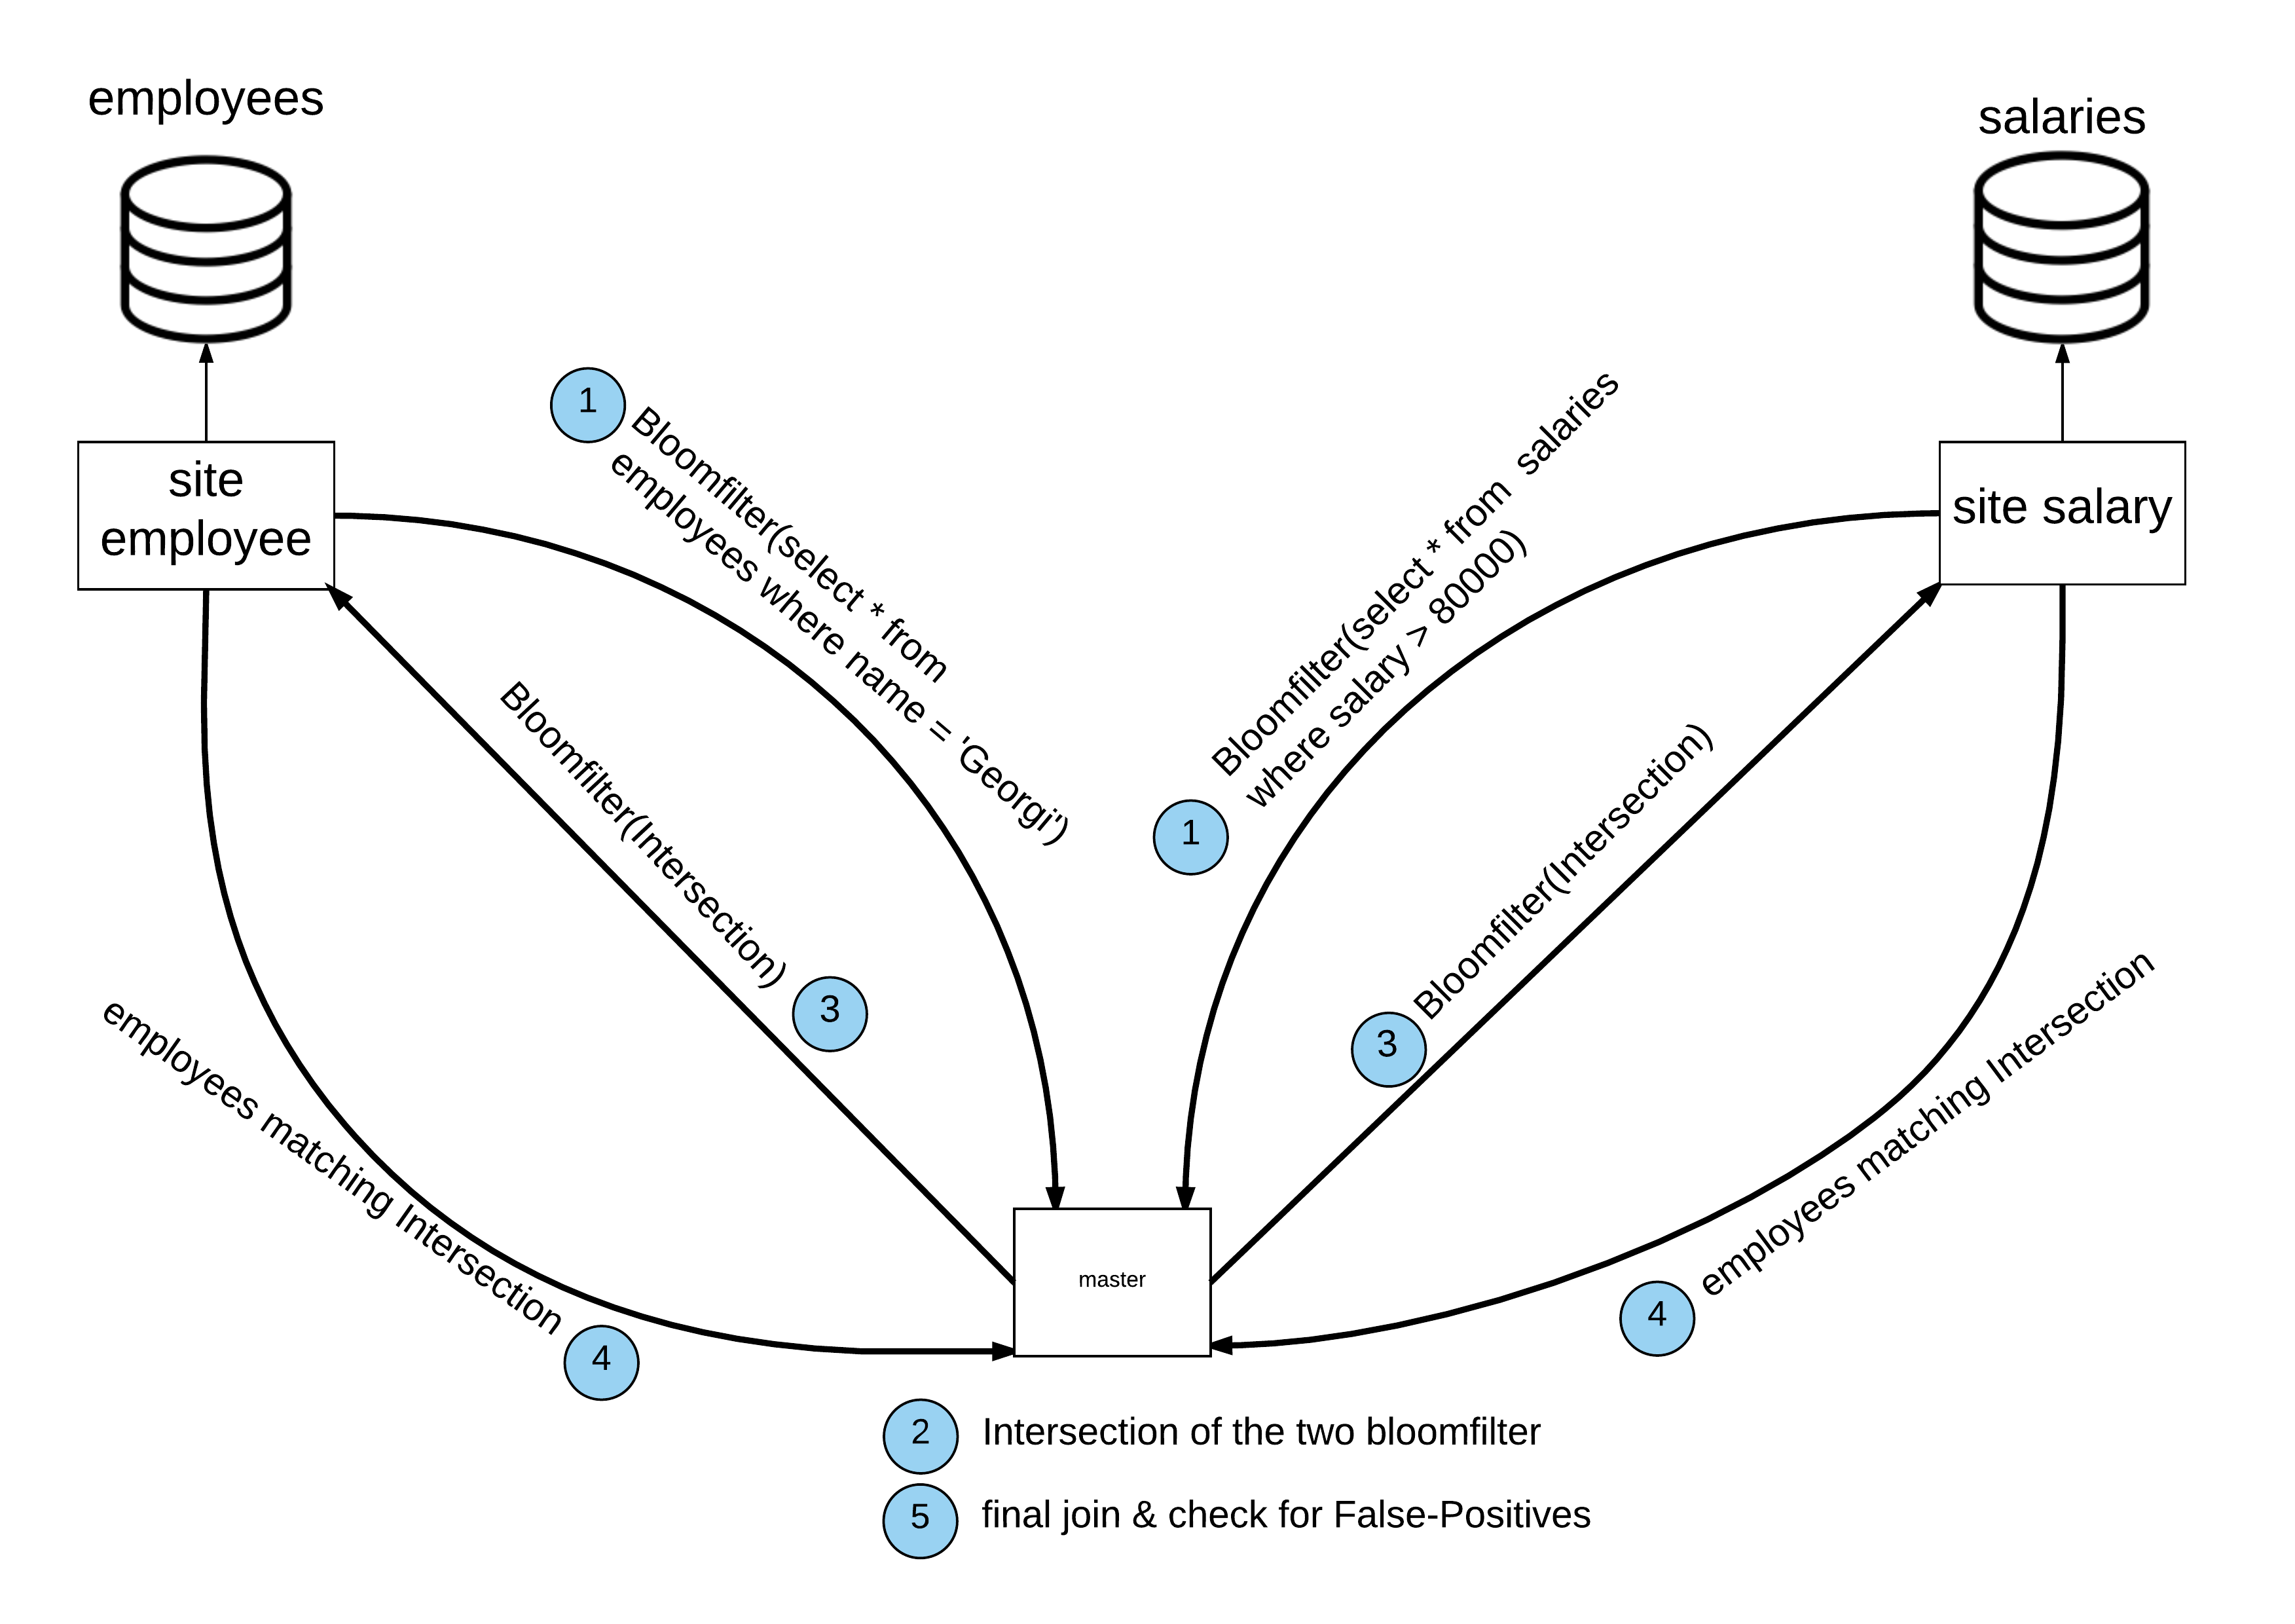
\includegraphics[scale=0.1]{res/architecture.png}
	\end{center}
	\caption{The architectural set-up of the experiment}
	\label{fig:architecture}
\end{figure}
Figure \ref{fig:architecture} shows an overview of our architectural set-up of the experiment. For our experiment we set the following SQL-queries, which were used on their corresponding tables within the databases:

\begin{itemize}
	\item[]  \textbf{S1}: \begin{verb}
		SELECT emp_no FROM employees WHERE first_name = 'Georgi'
	\end{verb}
	\item[]  \textbf{S2}: \begin{verb}
		SELECT emp_no FROM salaries WHERE salary > 80000.
	\end{verb}
\end{itemize}


The main steps of our concept are the following:
\begin{enumerate}
	\item The master site receives a Bitset from site employee and site salaries. These Bitset are a representation of a projection of all entries fulfilling the query \textbf{S1} on the employee side and \textbf{S2} on the salary side. Each BitSet is generated locally on each site with a identical Bloomfilter.
	\item An intersection between the two received Bitset is performed on the master site.
	\item The intersected Bitset is sent from the master to the two sides. it is used to check entries of the projection of 1 are in the intersected. This checking is done with the Bloomfilter.
	\item Entries matching the intersected Bitset will be send to the master side
	\item A actual join-process over employee.emp\_no = salary.emp\_no. is performed and the number of false-positives is evaluated.
	\end{enumerate}



One key aspect of any bloom filter implementation are the hash functions. They need to be independent and distribute uniformly. Both, equation \ref{set_to_1} and \ref{false_positive}, are only true for such hash functions. We decided to implement a universal class of hash functions. This allows us to define the number of hash functions to be used at the start and then we can choose those functions from our class. We used the same method as seen in Cormen (2009, p. 267), on designing a universal class of hash functions. As in the book described we chose a prime number p such that every key is smaller than p. Since we need to hash emp\_no in the bloom filter and the biggest emp\_no is smaller than 500'000, we chose $p = 500009$. We define two sets $\mathbb{Z}_p$ and $\mathbb{Z}_p^*$. $\mathbb{Z}_p$ denotes the set $\{0,1,...,p-1\}$ and $\mathbb{Z}_p^*$ denotes $\{1,2,...,p-1\}$. Then we can define a hash function with $a \in \mathbb{Z}_p^* \text{ and } b \in \mathbb{Z}_p$
\begin{equation}
	h_{ab}(k) = ((ak + b) \mathrel{mod} p) \mathrel{mod} m.
\end{equation}
In our case, $p = 500009$ and m is the size of the bloom filter. This is one hash function of the family of hash functions defined by
\begin{equation}
\mathbb{H}_{pm} = \{h_{ab} \mathrel{:} a \in \mathbb{Z}_p^* \text{ and } b \in \mathbb{Z}_p\}.
\end{equation}
This means, for every hash function we simply choose a and b randomly from their sets to create $h_{ab}$.\\\\

\section{Implementation}
DO WE NEED THIS SECTION? DO WE WANT TO SHOW SOME OF THE IMPLEMENTATIOS-TECHNIQUES WE USED. MAYBE DEPENDS ON LENGTH OF OTHER SECTIONS? (- TRICK HOW WE COUNT FALSE POSITIVE THAT WE DONT NEED TO COMPARE AGAIN)
In this section we want to present some details of our implementation with focus on interesting parts.

\subsection{Counting False Positive}
When we perform the join as seen in figure REFERENCE TO FIGURE, in step INSERT NUMBER both sites return the join-matching tuples. Lets define these results as two sets $S_{emp}$ from site employee and $S_{sal}$ from site salary. We claim that if the emp\_no of a tuple in $S_{emp}$ is also in $S_{sal}$, then it cannot be a false positive. In other words, whenever a tuple in $S_{emp}$ has a emp\_no that does not exist in $S_{sal}$ and vice versa, it must be a false positive. \\
To show this, we first consider what sort of emp\_no these sets potentially can contain. Lets consider site employee. We check all emp\_no returned from the query
\begin{verbatim}
SELECT emp_no FROM employees WHERE first_name = 'Georgi'
\end{verbatim}
against the composed bloom filter. Hence, all tuples in $S_{emp}$, true matches and false positives, have a emp\_no from a employee with $first_name = Georgi$. Same is true for $S_{sal}$ just with emp\_no from this query 
\begin{verbatim}
SELECT emp_no FROM salaries WHERE salary > 80000.
\end{verbatim}
Now, we assume there exists a emp\_no which is in $S_{emp}$ and in $S_{sal}$ and \emph{is} a false positive. By construction a emp\_no in $S_{emp}$ is from a tuple with $first\_name = Georgi$ and a emp\_no from $S_{sal}$ is form a tuple with $salary > 80'000$. Hence, a emp\_no which is in $S_{emp}$ and in $S_{sal}$ corresponds to a employee with $first\_name = Georgi$ and $salary > 80'000$. This is a true join match and therefore cannot be a false positive.


\section{Evaluation}
We ran our program with multiple inputs to see whether the expected values correlate with the data from our experiment. The data depends on the number of data points we insert in site employee ($n_{emp}$) and site salary ($n_{sal}$), the size of the bloom filter denoted as m and the number of hash functions denoted as k. As we kept the queries consistent, $n_{emp} \text{ and } n_{sal}$ stayed constant and we experimented with m and k. The queries we used returned $n_{emp} = 253$ and $n_{sal} = 17416$. To get reasonable expected values for the number of ones in a bloom filter, we chose m from 1'000 to 101'000 in steps of 2'000 and k from 1 to 31 in steps of 10.
In this section, we present our findings based on three figures. You can find all of our comparison graphs in the appendix.
\begin{figure}[ht]
	\begin{center}
		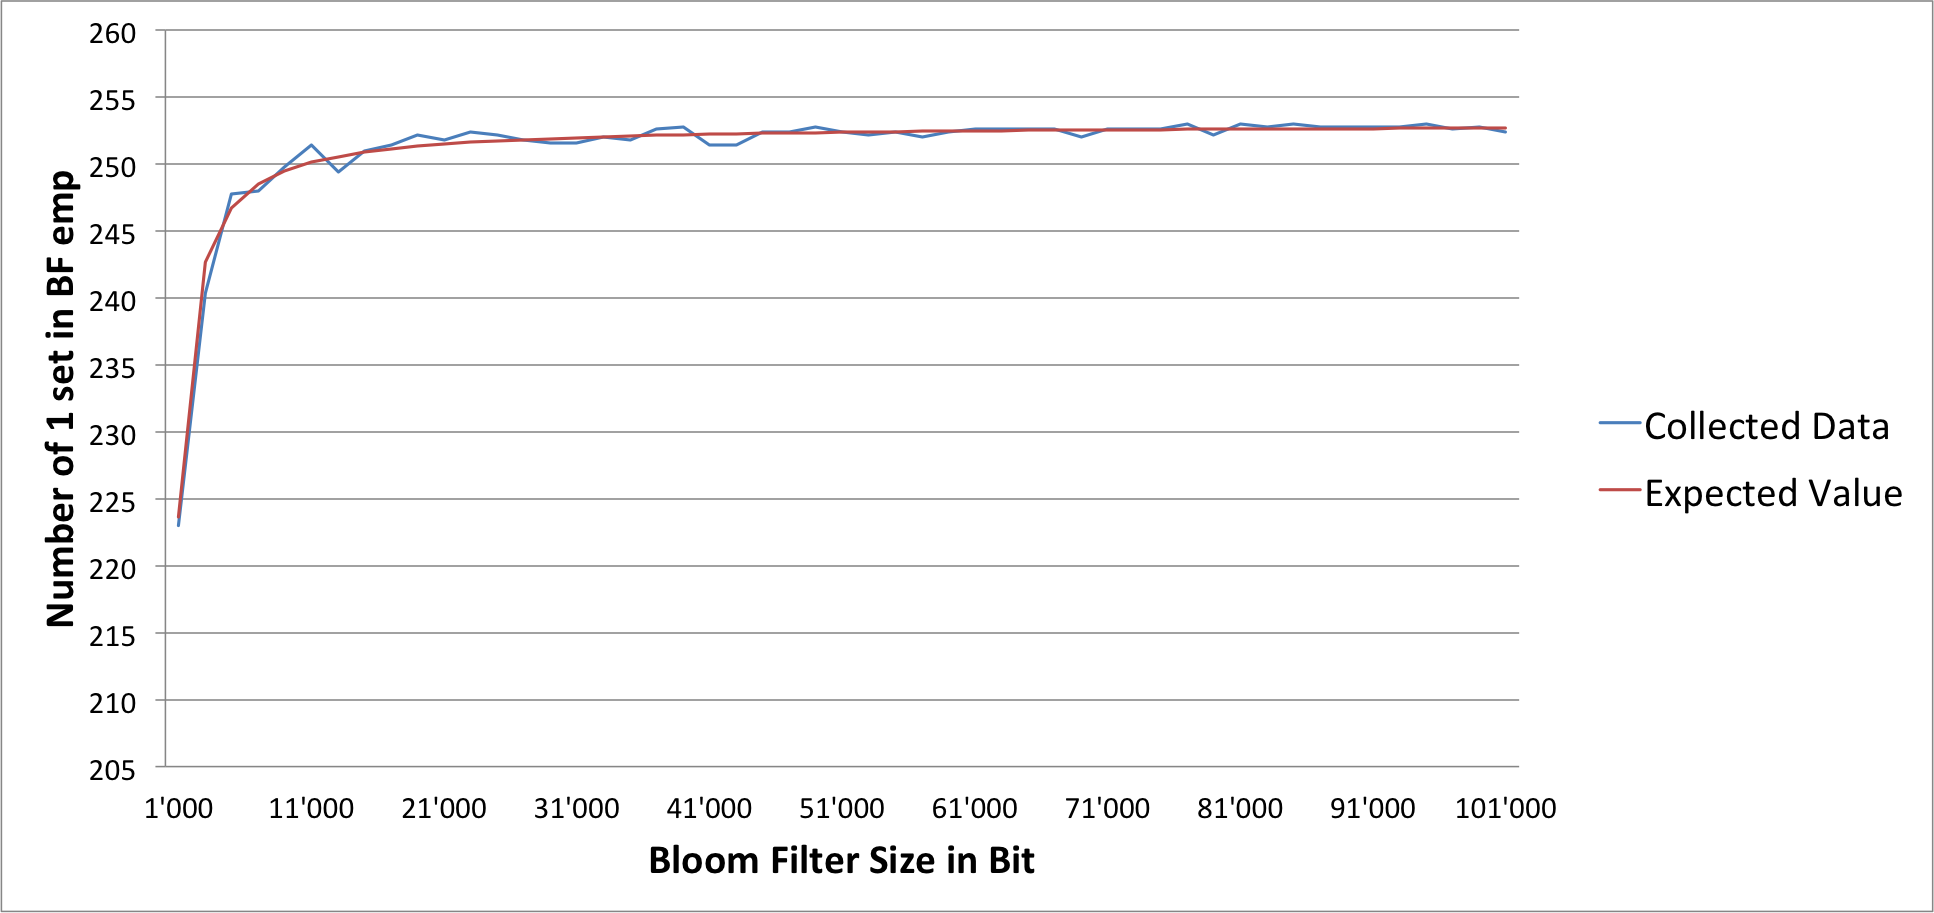
\includegraphics[scale=0.4]{res/1-emp.png}
	\end{center}
	\caption{Number of ones set in bloom filter from site employees - expected and measure in experiment with k = 1.}
	\label{fig:eval1}
\end{figure}\\
In figure \ref{fig:eval1}, we can clearly see that the number of ones in the bloom filter from the site employee in step 1 in our experiment behaves as we expected in equation \ref{set_to_1}. Figure \ref{fig:eval1} only verifies our expectation when using only one hash function (k=1), but we can see this verification for all expectations about the number of ones in a non-composed bloom filter.
\begin{figure}[ht]
	\begin{center}
		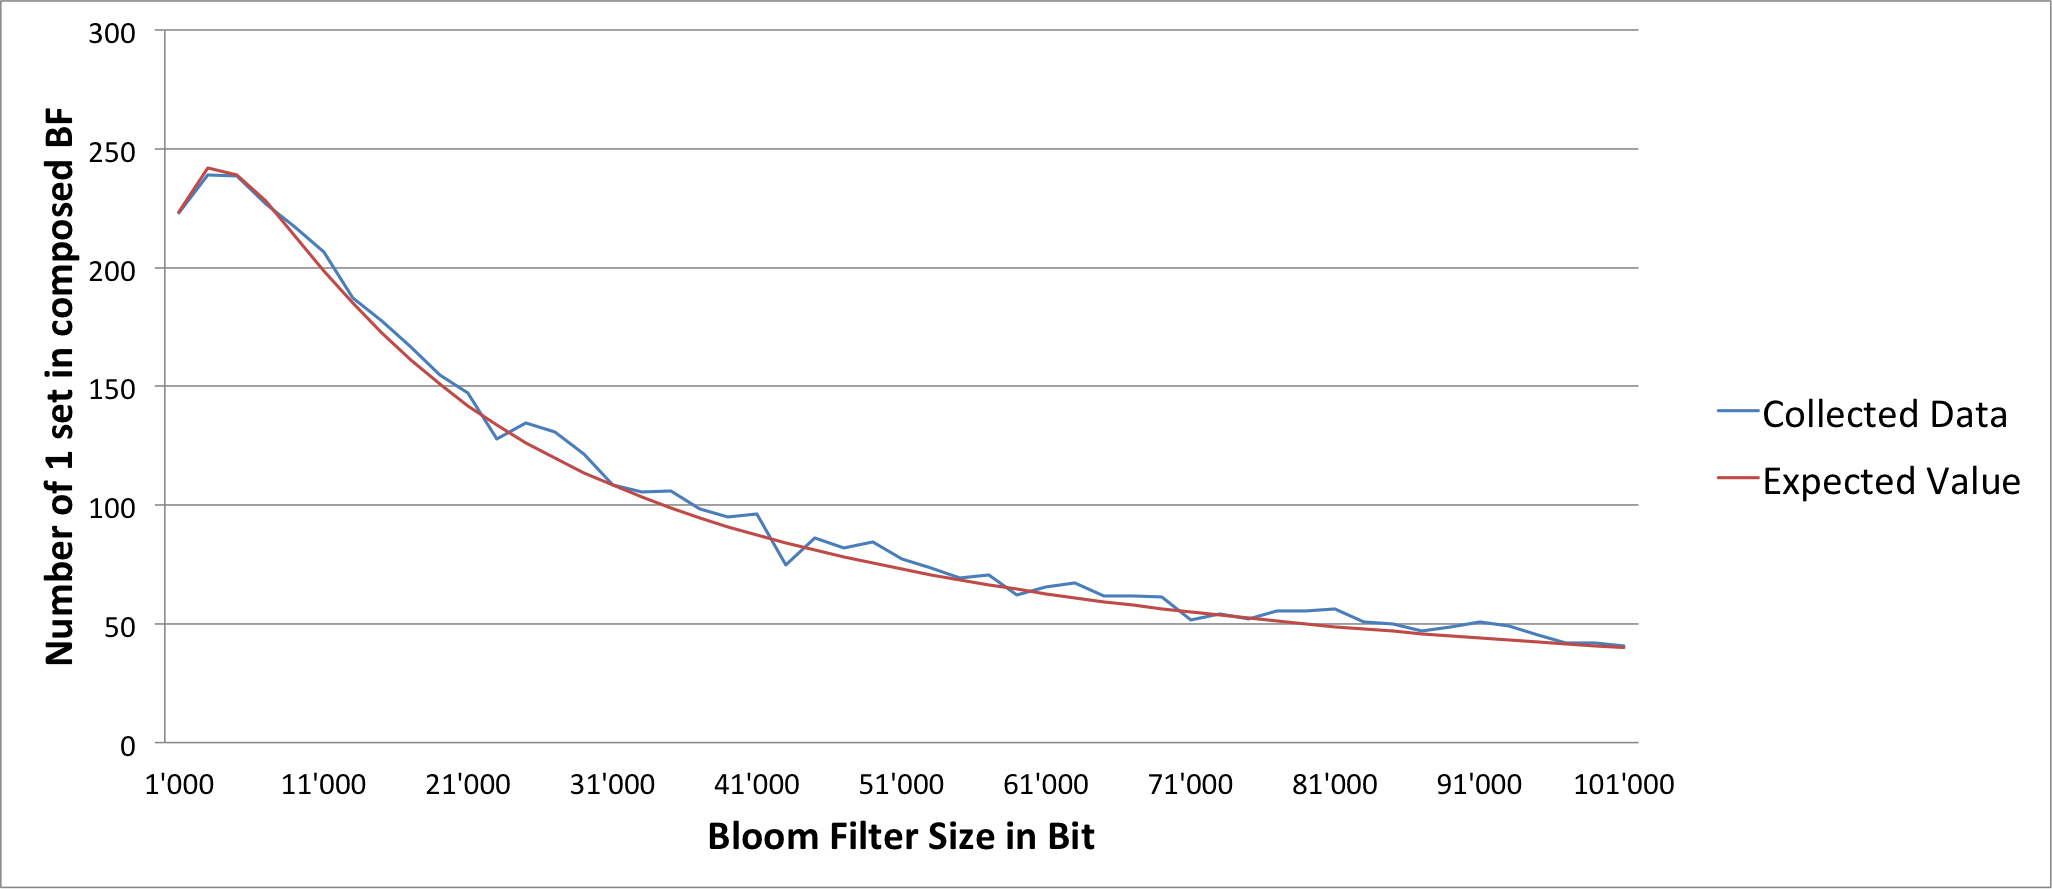
\includegraphics[scale=0.4]{res/1-composed.png}
	\end{center}
	\caption{Number of ones set in bloom filter from site employees - expected and measure in experiment with k = 1.}
	\label{fig:eval2}
\end{figure}
Same is true for the our expectation for the number of ones in the composed bloom filter. Figure \ref{fig:eval2} shows, again with k=1, that our expectation in equation \ref{set_to_1_composed} is also correct.


\section{Conclusion}

\bibliography{refs}
\bibliographystyle{abbrv}
\end{document}